
\documentclass{article}
\usepackage[utf8]{inputenc}
\usepackage{graphicx}
\usepackage{listings}
\usepackage{xcolor}
\usepackage{float}  % Add float package to control figure placement
\usepackage{amsmath}

\title{08a Servo Motors Intro}
\author{Nicholas Bruzzese}
\date{\today}

\definecolor{dkgreen}{rgb}{0,0.6,0}
\definecolor{gray}{rgb}{0.5,0.5,0.5}
\definecolor{mauve}{rgb}{0.58,0,0.82}

\lstset{frame=tb,
	language=Python,
	aboveskip=3mm,
	belowskip=3mm,
	showstringspaces=false,
	columns=flexible,
	basicstyle={\small\ttfamily},
	numbers=none,
	numberstyle=\tiny\color{gray},
	keywordstyle=\color{blue},
	commentstyle=\color{dkgreen},
	stringstyle=\color{mauve},
	breaklines=true,
	breakatwhitespace=true,
	tabsize=3
}

\begin{document}
	
	\maketitle
	
	\section*{Understanding PWM and Servo Control}
	
	Pulse Width Modulation (PWM) is a technique where the width of a pulse is varied while keeping the frequency constant. This method is essential for controlling servo motors, as the duration of the pulse determines the position of the servo's shaft.
	
	In a typical setup, a 50Hz PWM signal (period of 20ms) is used:
	\begin{itemize}
		\item \textbf{0° Position}: A 1ms pulse width (5\% duty cycle) positions the servo at 0 degrees.
		\item \textbf{90° Position}: A 1.5ms pulse width (7.5\% duty cycle) positions the servo at 90 degrees.
		\item \textbf{180° Position}: A 2ms pulse width (10\% duty cycle) positions the servo at 180 degrees.
	\end{itemize}
	
	By adjusting the pulse width within this range, you can set the servo to any desired angle between 0° and 180°.
	
	\section*{Setting Up Your Raspberry Pi with a Servo Motor}
	
	\subsection*{Hardware Connections}
	
	\textbf{Servo Motor Wires}:
	\begin{itemize}
		\item \textbf{Red (VCC)}: Connect to the 3.3V pin on the Raspberry Pi.
		\item \textbf{Brown/Black (GND)}: Connect to a ground (GND) pin on the Raspberry Pi.
		\item \textbf{Yellow/Orange (Signal)}: Connect to a GPIO pin (e.g., GPIO17, pin 11).
	\end{itemize}
	
	Optional: For added safety, place a $\sim$1k$\Omega$ resistor between the signal wire and the GPIO pin.
	
	\textbf{Note}: If the servo doesn't operate correctly, it might be due to insufficient power. In such cases, consider using an external power source (4--6V) for the servo.
	
	\subsection*{Software Configuration}
	
	\textbf{Install the RPi.GPIO Library}:
	\begin{lstlisting}[language=bash]
		sudo apt-get update
		sudo apt-get install python3-rpi.gpio
	\end{lstlisting}
	
	\section*{Wiring Diagram}
	This is a simple setup:
	
	\begin{figure}[H]
		\centering
		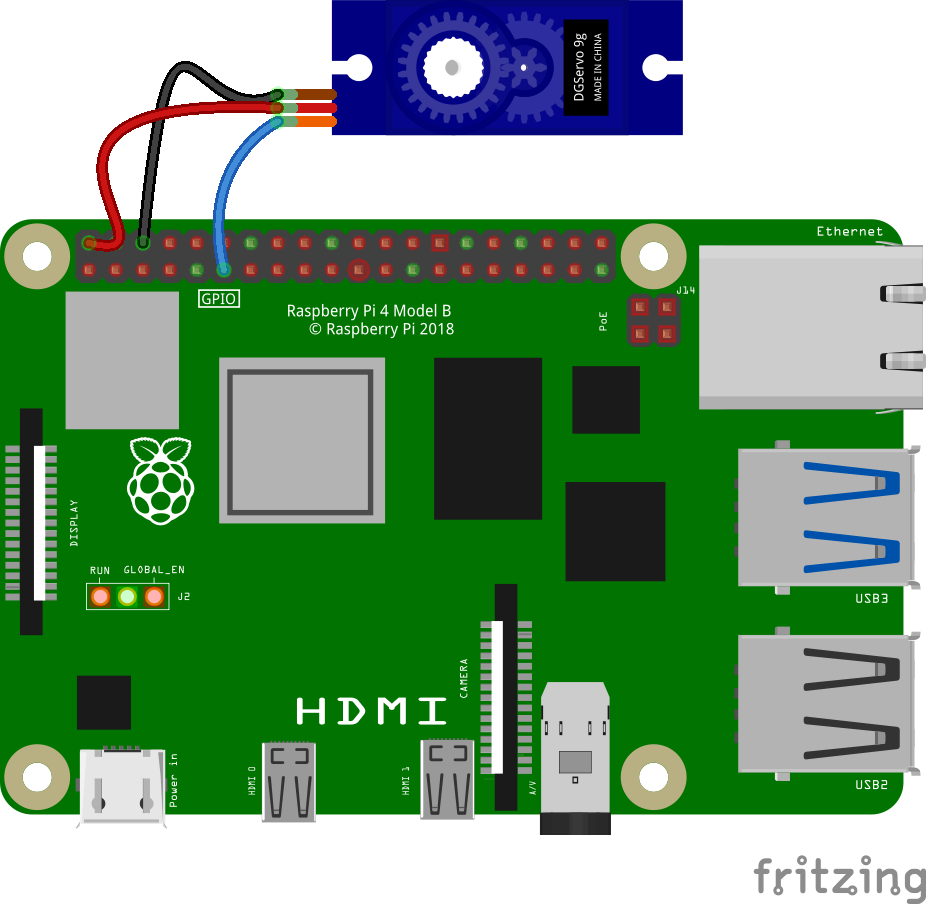
\includegraphics[width=0.7\textwidth]{08a-servo-motors-intro.png} % Adjust width to 80% of text width
		\caption{Wiring Diagram}
	\end{figure}
	
	\newpage
	\textbf{Python Script to Control the Servo}:
	
	Create a Python script (e.g., \texttt{servomotor.py}) with the following content:
	
	\begin{lstlisting}[language=python]
		import RPi.GPIO as GPIO
		import time
		
		servoPIN = 17
		GPIO.setmode(GPIO.BCM)
		GPIO.setup(servoPIN, GPIO.OUT)
		
		p = GPIO.PWM(servoPIN, 50)  # GPIO 17 for PWM with 50Hz
		p.start(2.5)  # Initialization
		
		try:
			while True:
			p.ChangeDutyCycle(5)    # Move to 0 degrees
			time.sleep(0.5)
			p.ChangeDutyCycle(7.5)  # Move to 90 degrees
			time.sleep(0.5)
			p.ChangeDutyCycle(10)   # Move to 180 degrees
			time.sleep(0.5)
			p.ChangeDutyCycle(7.5)  # Move back to 90 degrees
			time.sleep(0.5)
		except KeyboardInterrupt:
			p.stop()
			GPIO.cleanup()
	\end{lstlisting}
	
	\textbf{Running the Script}:
	
	Execute the script using Python:
	\begin{lstlisting}[language=bash]
		python3 servomotor.py
	\end{lstlisting}
	
	This script will cycle the servo motor through 0°, 90°, and 180° positions. Adjust the \texttt{ChangeDutyCycle} values to set specific angles as needed.
	
\end{document}
